% Beamtime April 2015
Further experiments were carried out to increase the cleanliness of the \textit{h}-BN on the polycrystalline copper foil. To reduce the amount of elements coming from the body of the foil, it is repeatedly sputtered and annealed to temperatures as high as \SI{800}{\celsius}. This may have also an improving influence on the grain size and amount of corrugation. Several attempts have been made which are described in summary below.
%%%%%%%%%%%%%%%%%%%%%%%%%%%%%%%%%%%%%%%%%%%%%%%%%%%%%%%%%%%%%%%%%%%%%%%%%%%%%%%%%%%%%%%%%%
\section{Characterization of clean copper foil}
\begin{itemize}
 \item After cleaning, the sample is investigated in STM. The foil shows a inhomogeneous topography, with parts of the sample showing very flat regions while others still remain heavily corrugated and not scan able in STM. 
 A first look onto the quite heterogeneous surface reveals flat areas with a typical roughness of $\approx \SI{70}{\pico\meter}$ exist (\autoref{fig:cu-foil-clean}). Areas with very large corrugations $\geq \SI{100}{nm}$ are hard to scan in STM and bad places for \textit{h}-BN growth. Although being flat, the polycrystalline foil shows a lot of unordered substrate steps and a dirty surface, covered with adsorbates imaged as small bright dots.
\end{itemize}
%%%%%%%%%%%%%%%%%%%%%%%%%%%%%%%%%%%%%%%%%%%%%%%%%%%%%%%

\begin{figure}[] \centering
%	\subfigure[Roughness $\approx \SI{60}{\pico\meter}$.]{%
%		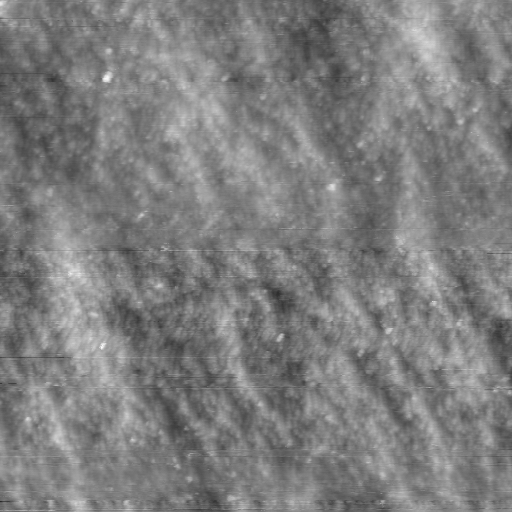
\includegraphics[width=0.45\textwidth]{./images/F150331-124839}
%		\label{fig:30-31.03}
%	}
	\subfigure[Cleaned copper foil before \textit{h}-BN growth. Surface shows many facets, the roughness is \SI{70}{\pico\meter}.]{%
		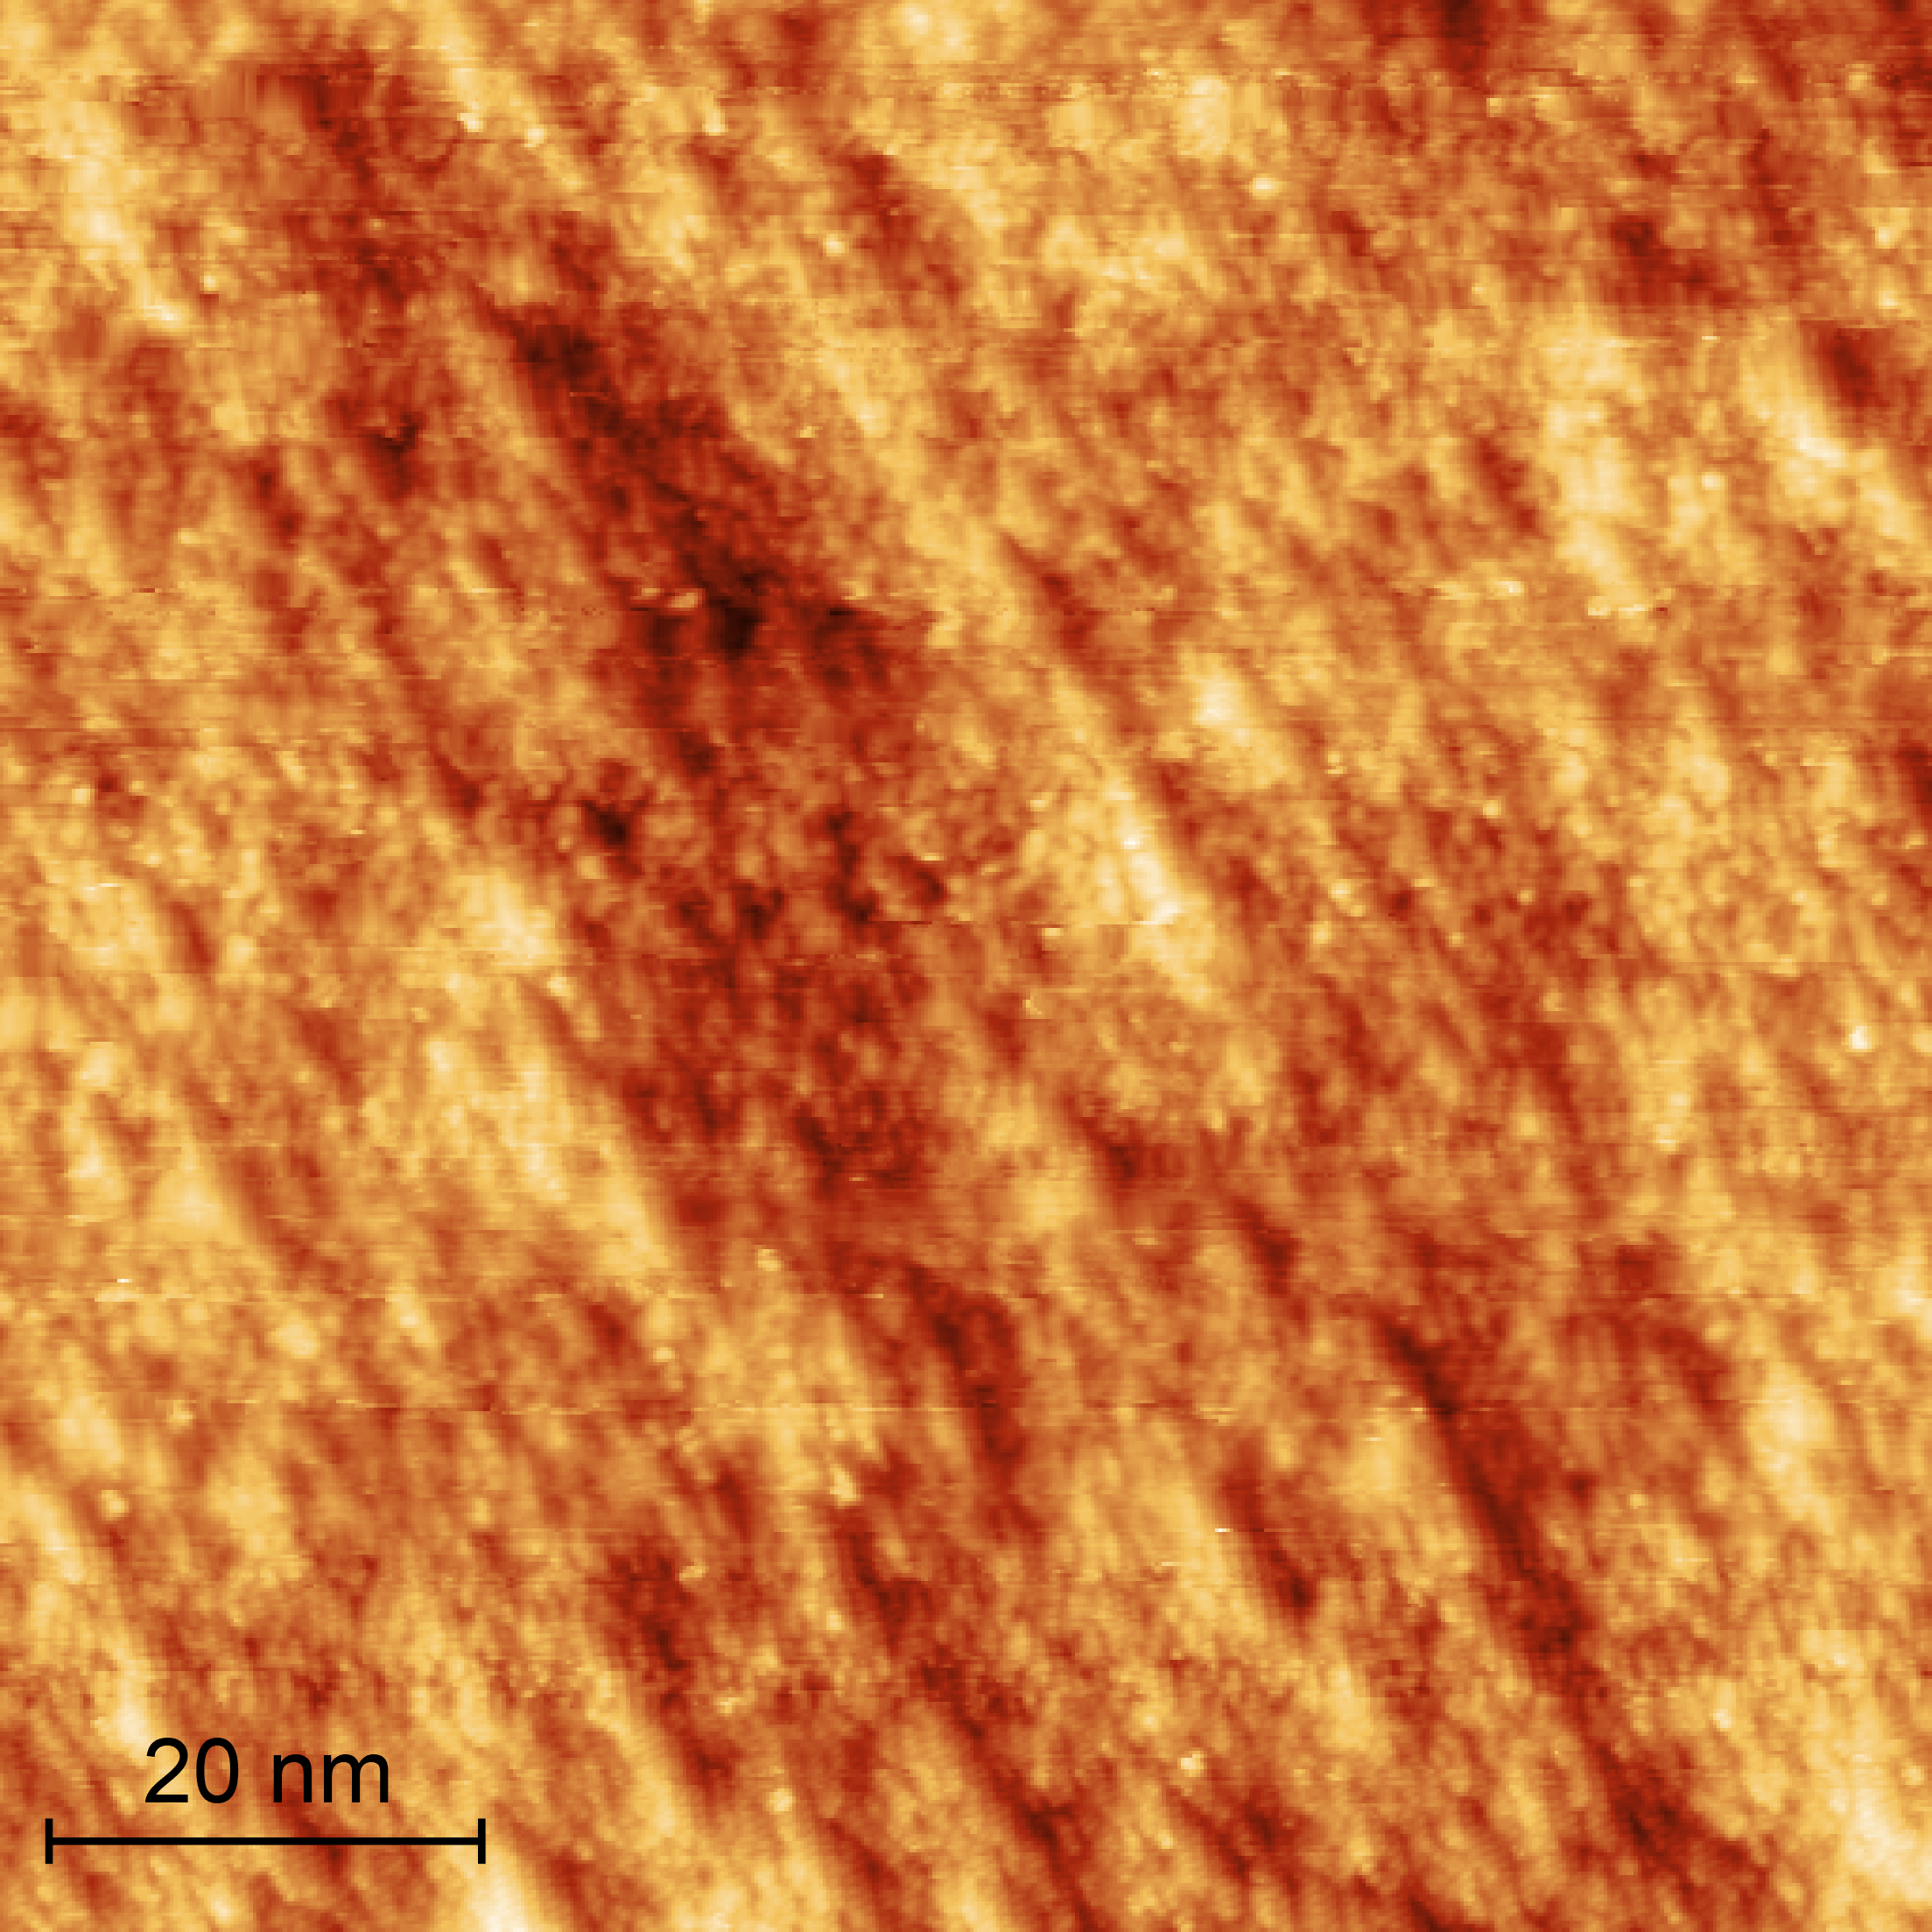
\includegraphics[width=0.5\textwidth]{./images/F150331-125720}
		\label{fig:cu-foil-clean-stm}
	} \quad
%	\subfigure[STM image after \SI{4.5}{\langmuir} of borazine dosage on a \SI{750}{\celsius} hot copper foil surface. A small \textit{h}-BN island can be seen (lower right) on a largely uncovered copper foil background.]{%
%		\includegraphics[width=0.45\textwidth]{./images/F150416-192611}
%		\label{fig:F150416-192611}
%	}
%	\subfigure[STM image of \SI{22}{\langmuir} borazine dosed on a \SI{800}{\celsius} hot copper-foil surface. Several large islands can be seen that grow over Cu-foil step edges. Inset shows coverage with \textit{h}-BN ad layer in blue.]{
%	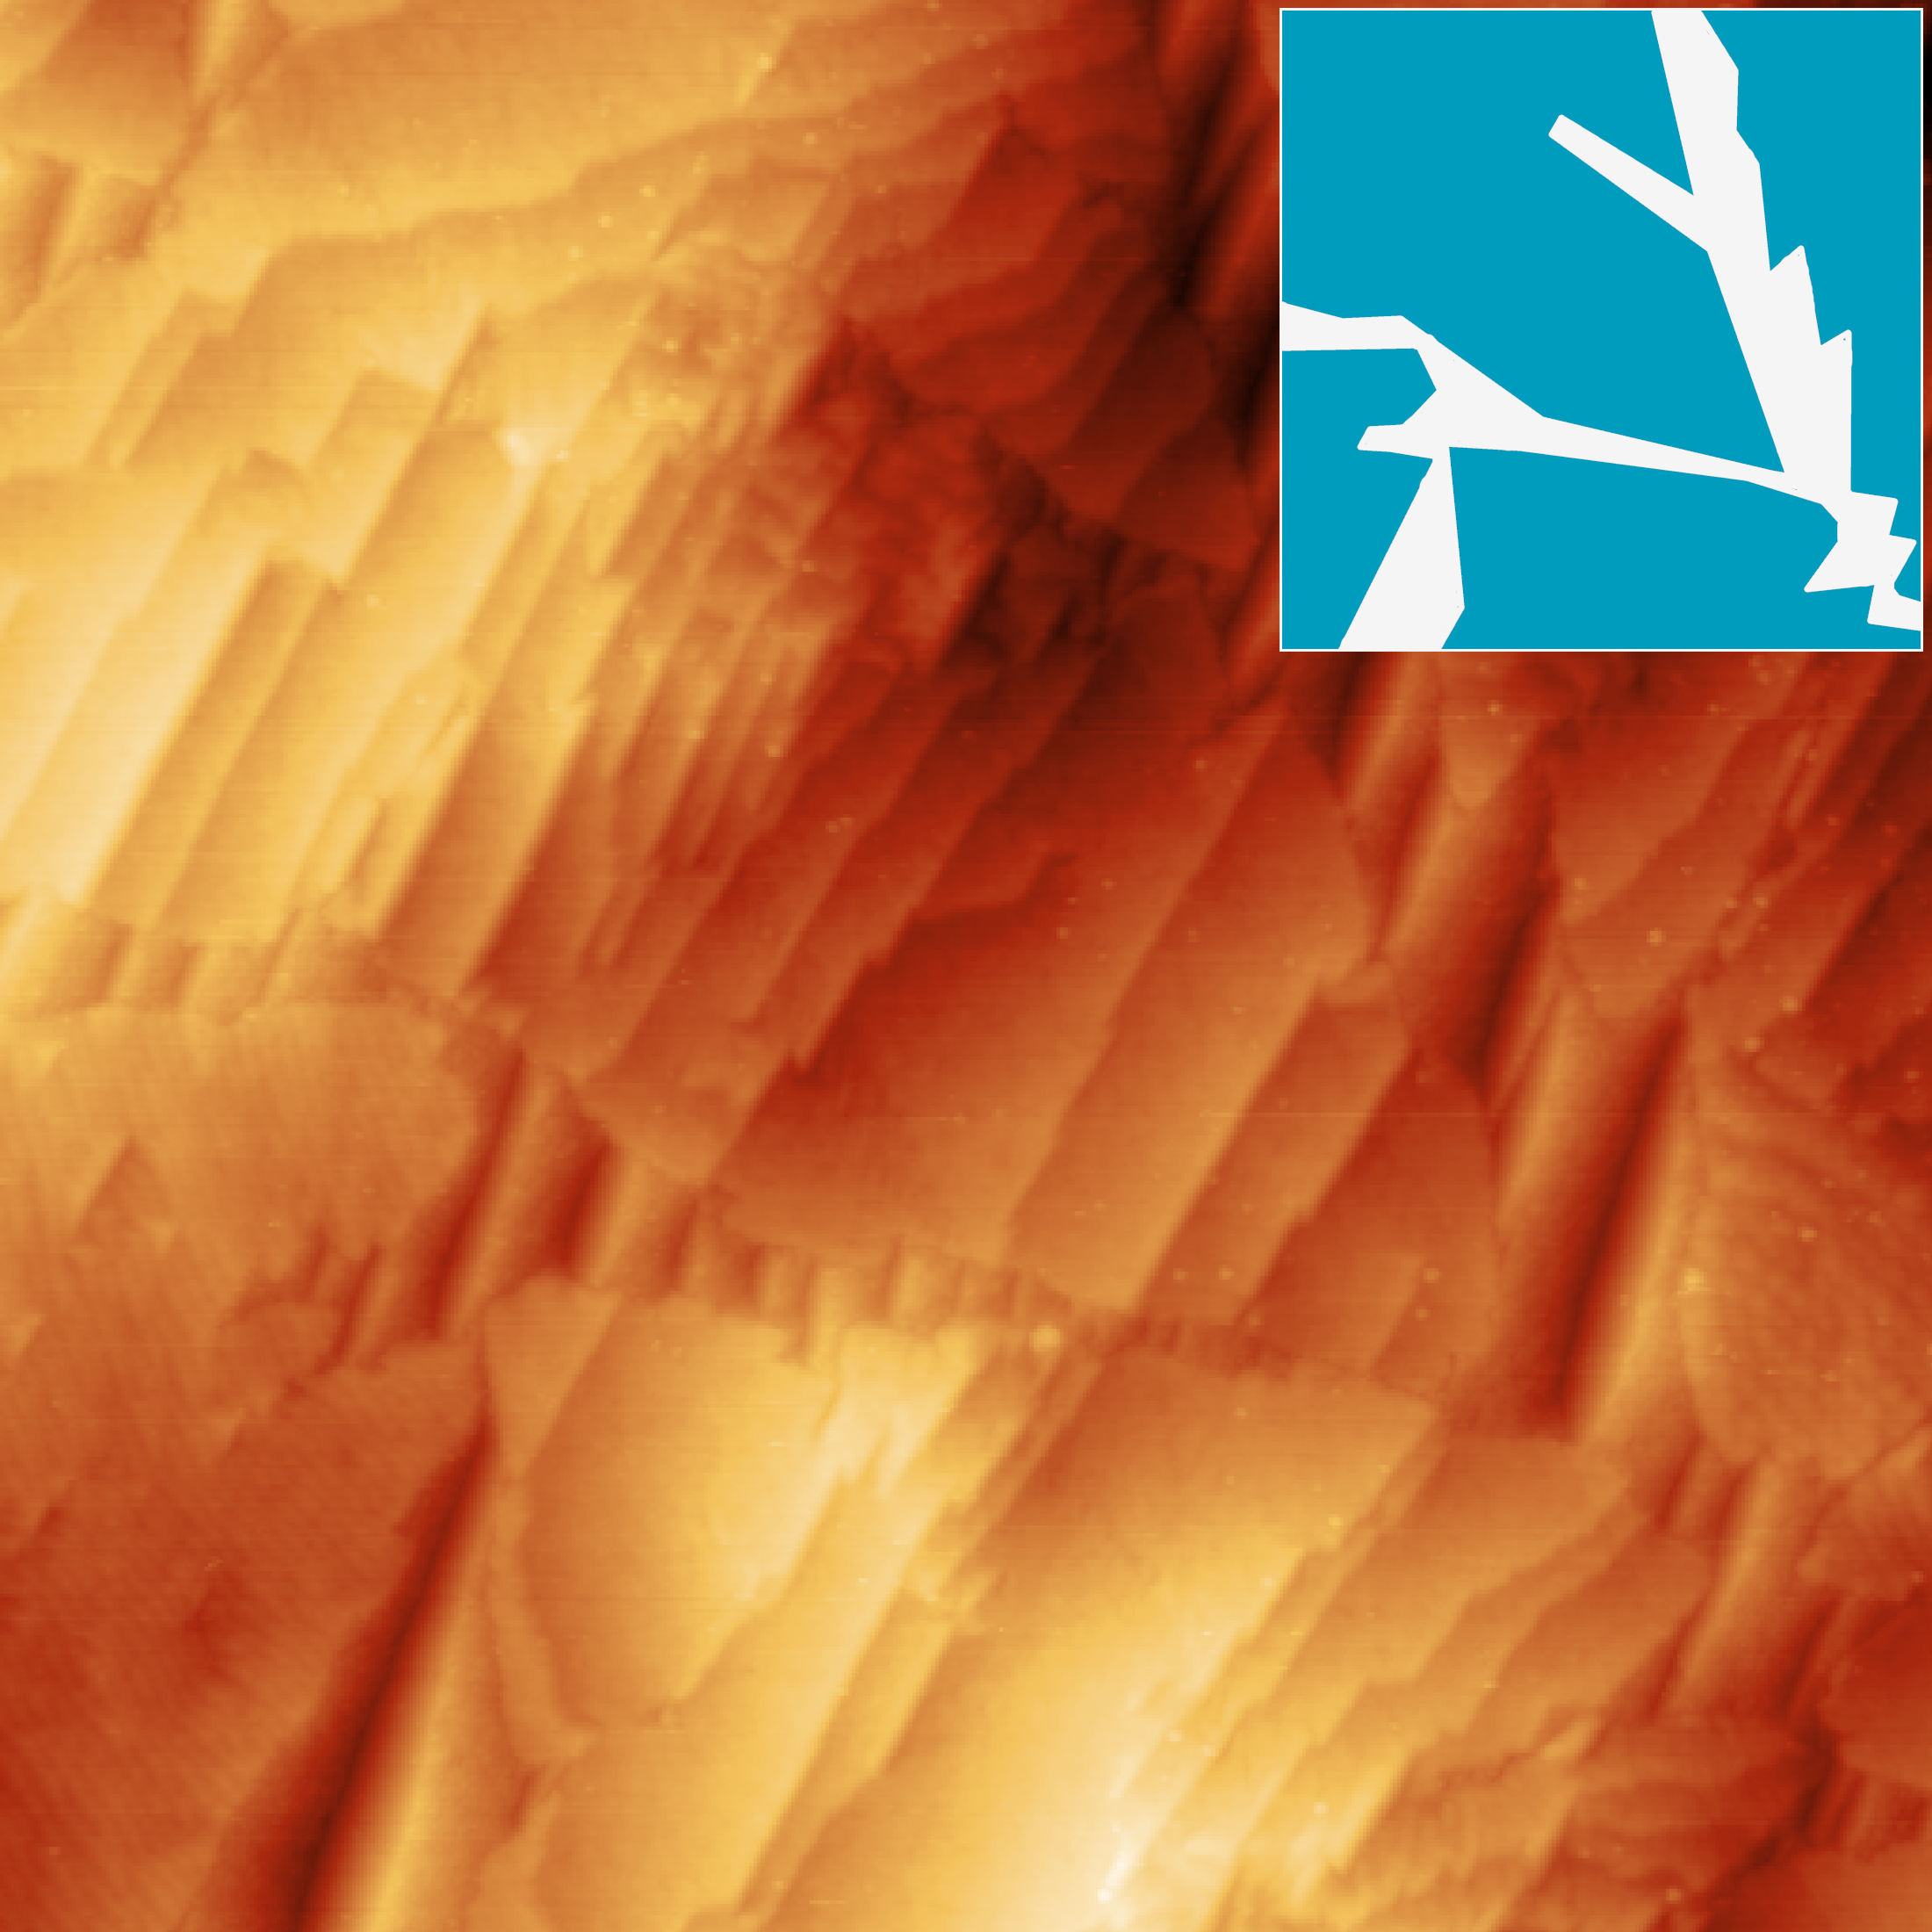
\includegraphics[width=0.35\textwidth]{./images/F150423-102732-with-inset}
%	\label{cu-foil-hBN-stm}
%}
	\subfigure[Typical height profile. the roughness is \SI{70}{\pico\meter}.]{%
	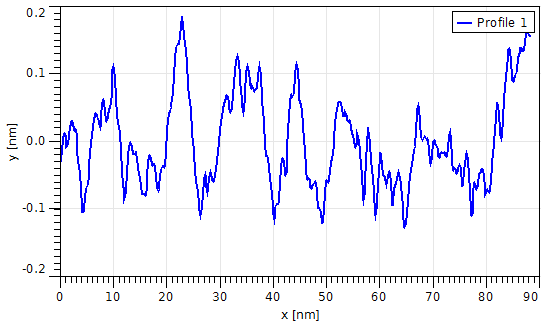
\includegraphics[width=0.5\textwidth]{./images/F150331-125720-profile}
	\label{fig:cu-foil-clean-profile}
}

\caption{Cu-foil \subref{fig:cu-foil-clean-stm} after repeated sputtering and annealing cycles. \subref{cu-foil-clean-profile} Height profile. Imaging parameters: \subref{fig:cu-foil-clean-stm} \SI{3.6}{\volt}, \SI{0.1}{\nano\ampere}, color scale \SIrange{0}{600}{\pico\meter}, Image width: \SI{88,6}{\nano \meter}, 
%	\subref{fig:F150416-192611} \SI{1}{\volt}, \SI{0.37}{\nano\ampere}, color scale \SIrange{0}{900}{\pico\meter}, Image width: \SI{44,3}{\nano \meter}.
%\subref{{cu-foil-hBN-stm}} \SI{4.7}{\volt}, \SI{0.2}{\nano\ampere}, color scale \SIrange{0}{7}{\nano\meter}, Image width: \SI{295}{\nano \meter}
	}
\end{figure}
%%%%%%%%%%%%%%%%%%%%%%%%%%%%%%%%%%%%%%%%%%%%%%%%%%%%%%%%%%%%%%%%%%%%%%%%%%%%%%%%%%%%%%%%%%
\begin{itemize}
 \item The foil was sputtered and annealed 4 times with temperatures of \SI{800}{\celsius}. Borazine was dosed at \SI{2e-7}{\milli \bar} for \SI{2.5}{\minute}. The sample was kept at \SI{750}{\celsius} for another 5 minutes after dosing. The sample was cooled down slowly. \autoref{fig:h-bn-overgrown-cu-1} shows some of the grown islands. The copper surface changes upon \textit{h}-BN growth and the terrace width increases below the \textit{h}-BN flakes. The typical faceting of the surface vanishes or can at least not be depicted because of the overgrowing \textit{h}-BN (\autoref{fig:h-bn-overgrown-cu-2}). 
\end{itemize}
% -----------BILDER ---- DISKUSSION: 21.04
%\begin{figure}
% \centering
% 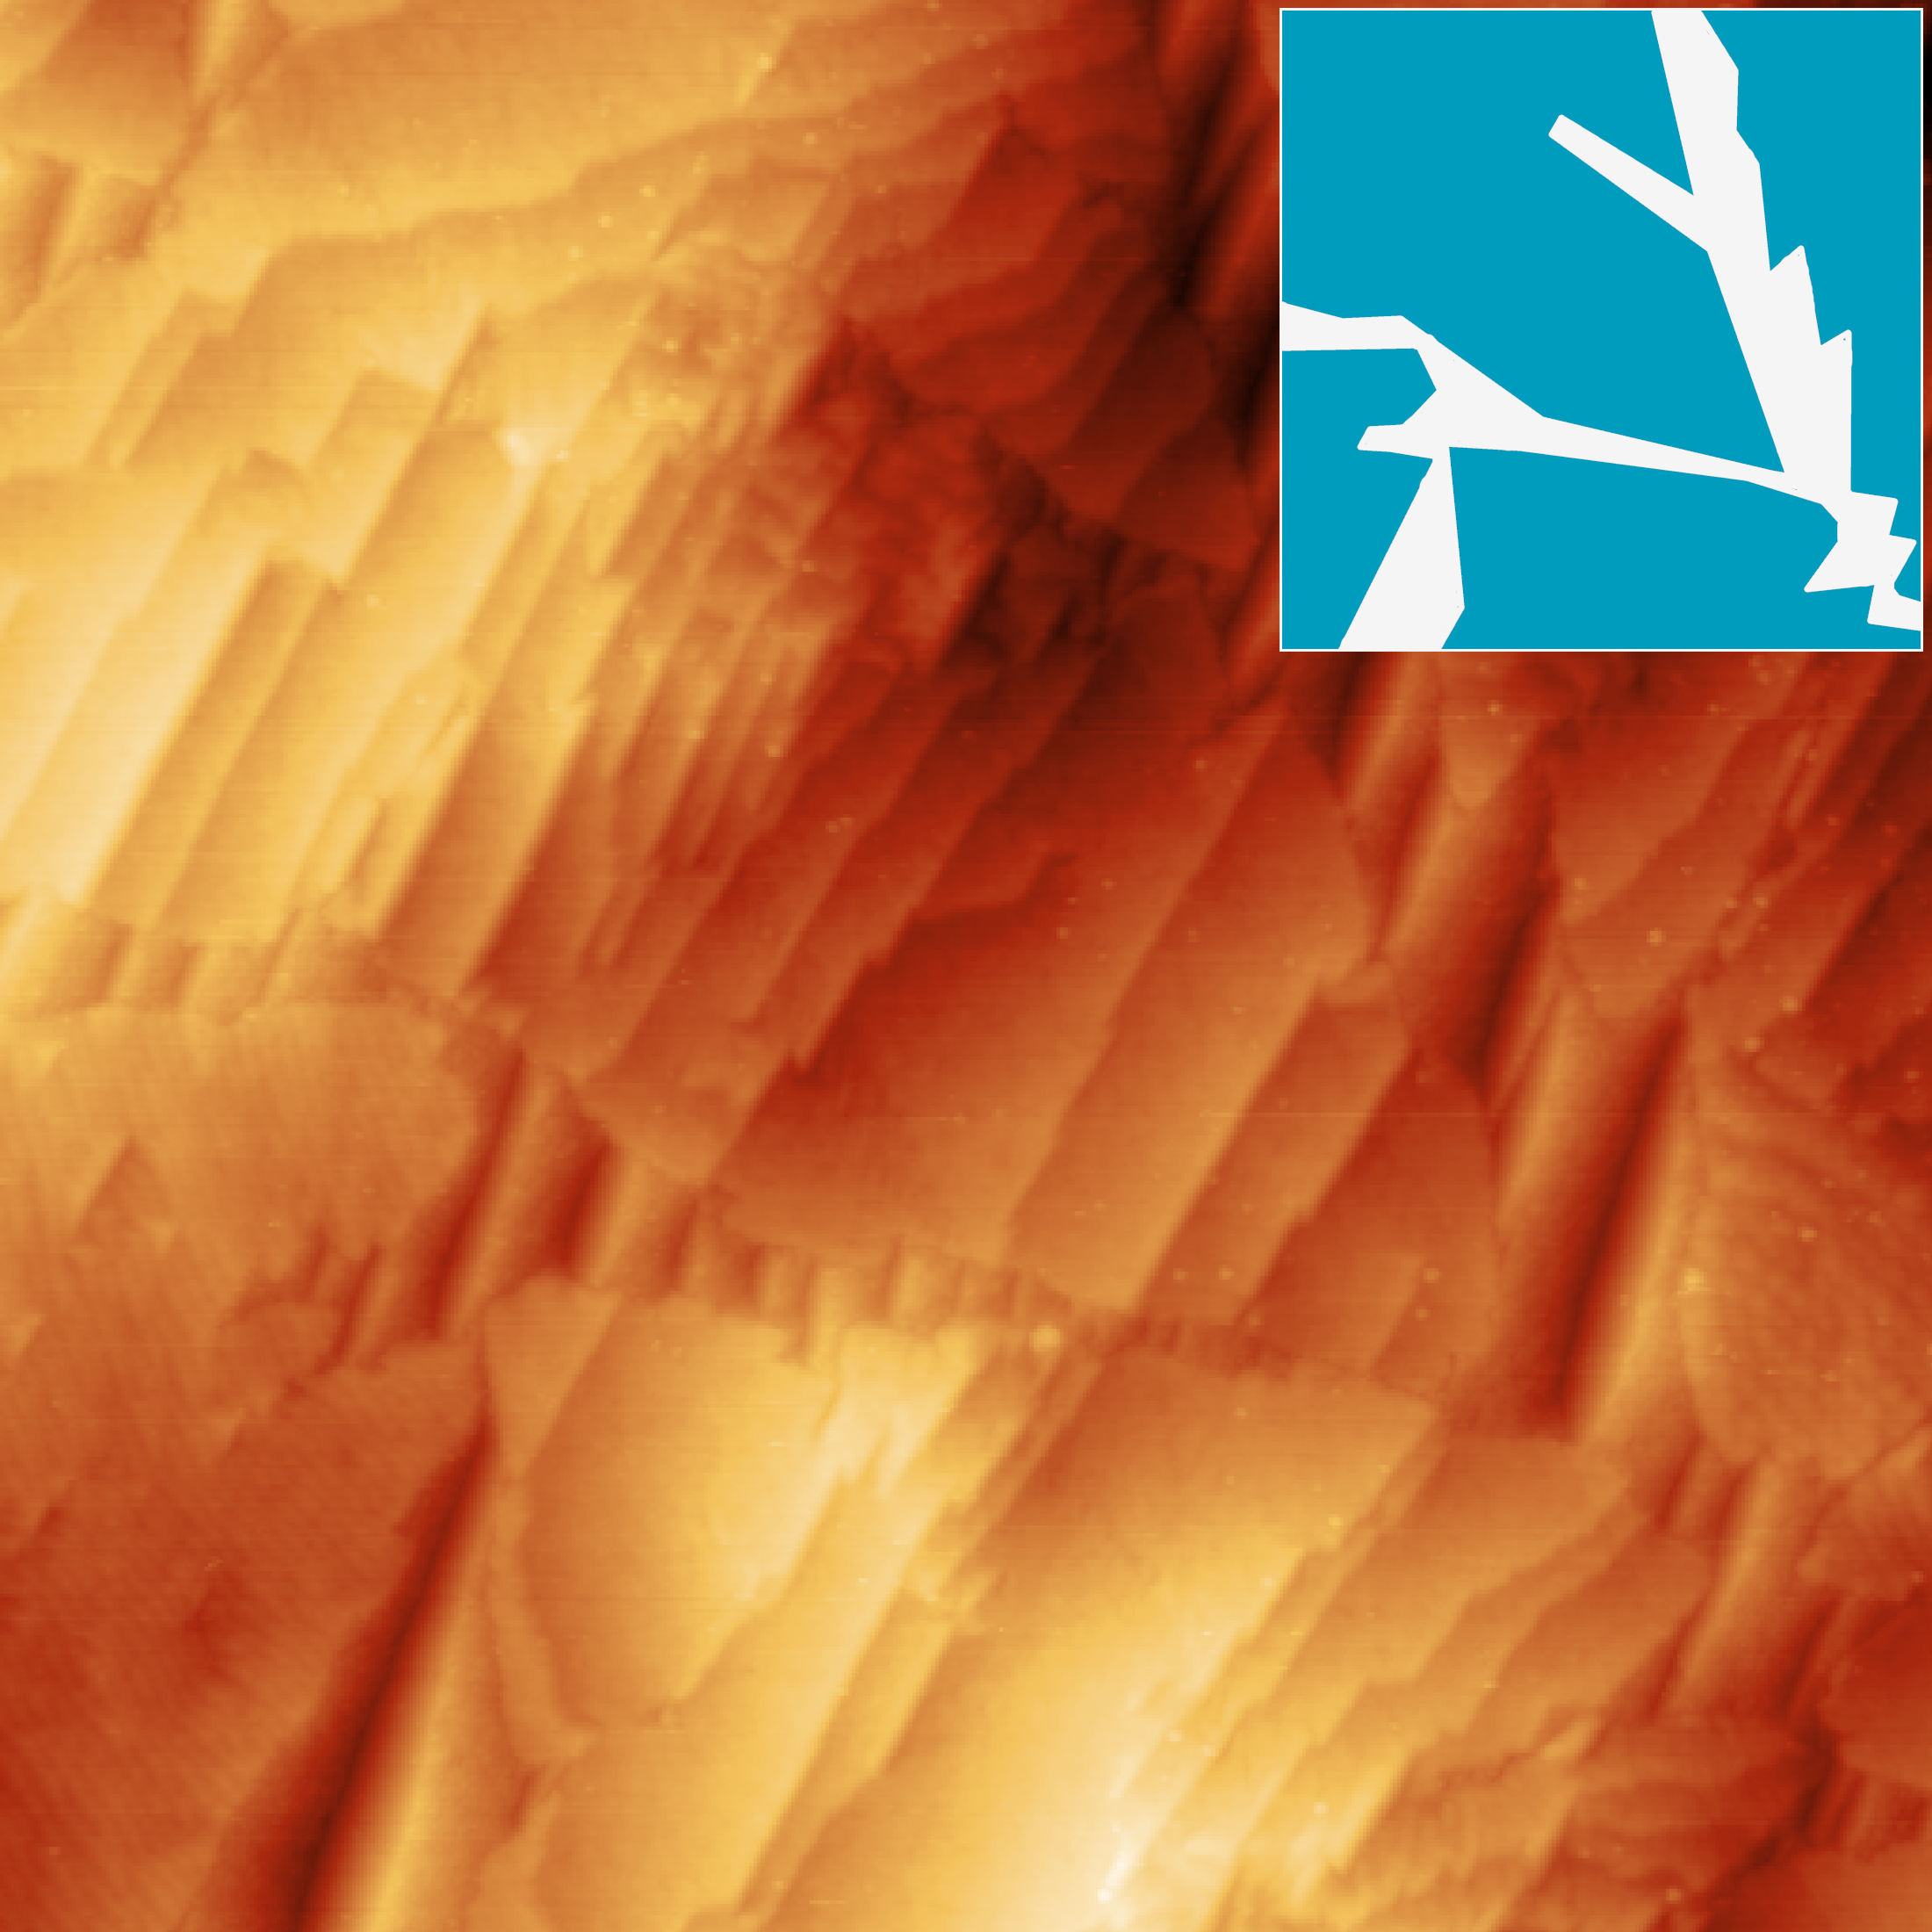
\includegraphics[width=0.7\textwidth]{./images/F150423-102732-with-inset}
% \caption{}
%\end{figure}
%%%%%%%%%%%%%%%%%%%%%%%%%%%%%%%%%%%%%%%%%%%%%%%%%%%%%%%%%%%%%%%%%%%%%%%%%%%%%%%%%%%%%%%%%%
%\begin{figure}
% \centering
%\subfigure[]{%
%	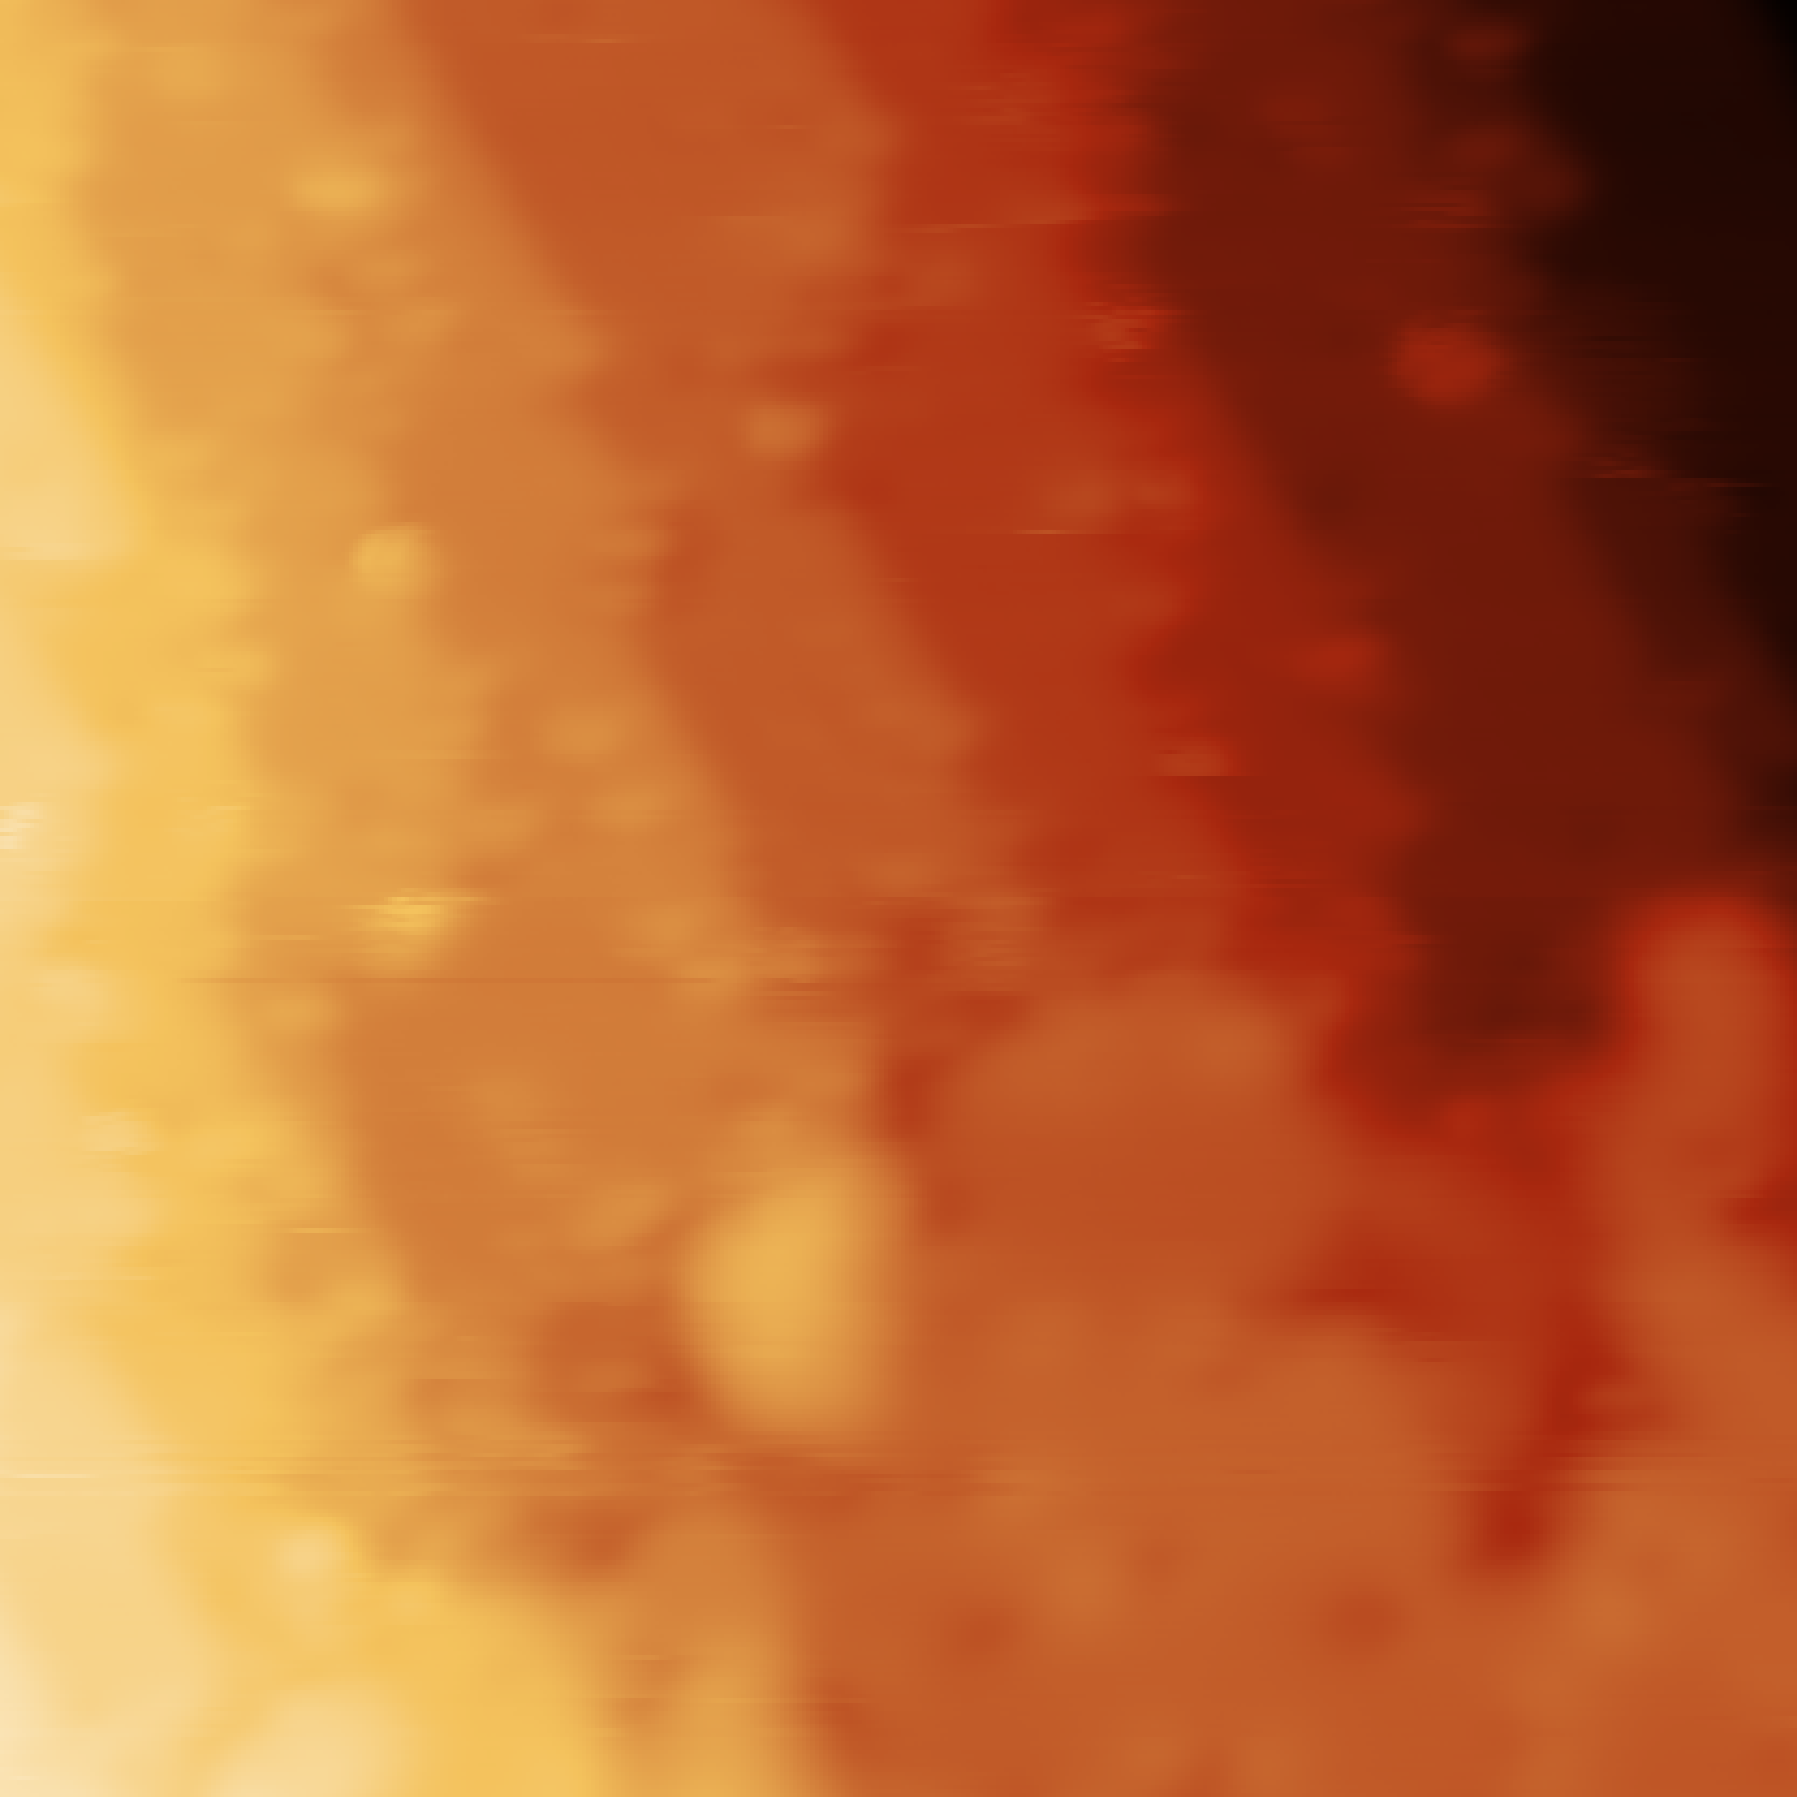
\includegraphics[width=0.45\textwidth]{./images/F150416-192611-detail1.png}
%	\label{fig:h-bn-overgrown-cu-1}
%} \quad %
%\subfigure[]{%
%	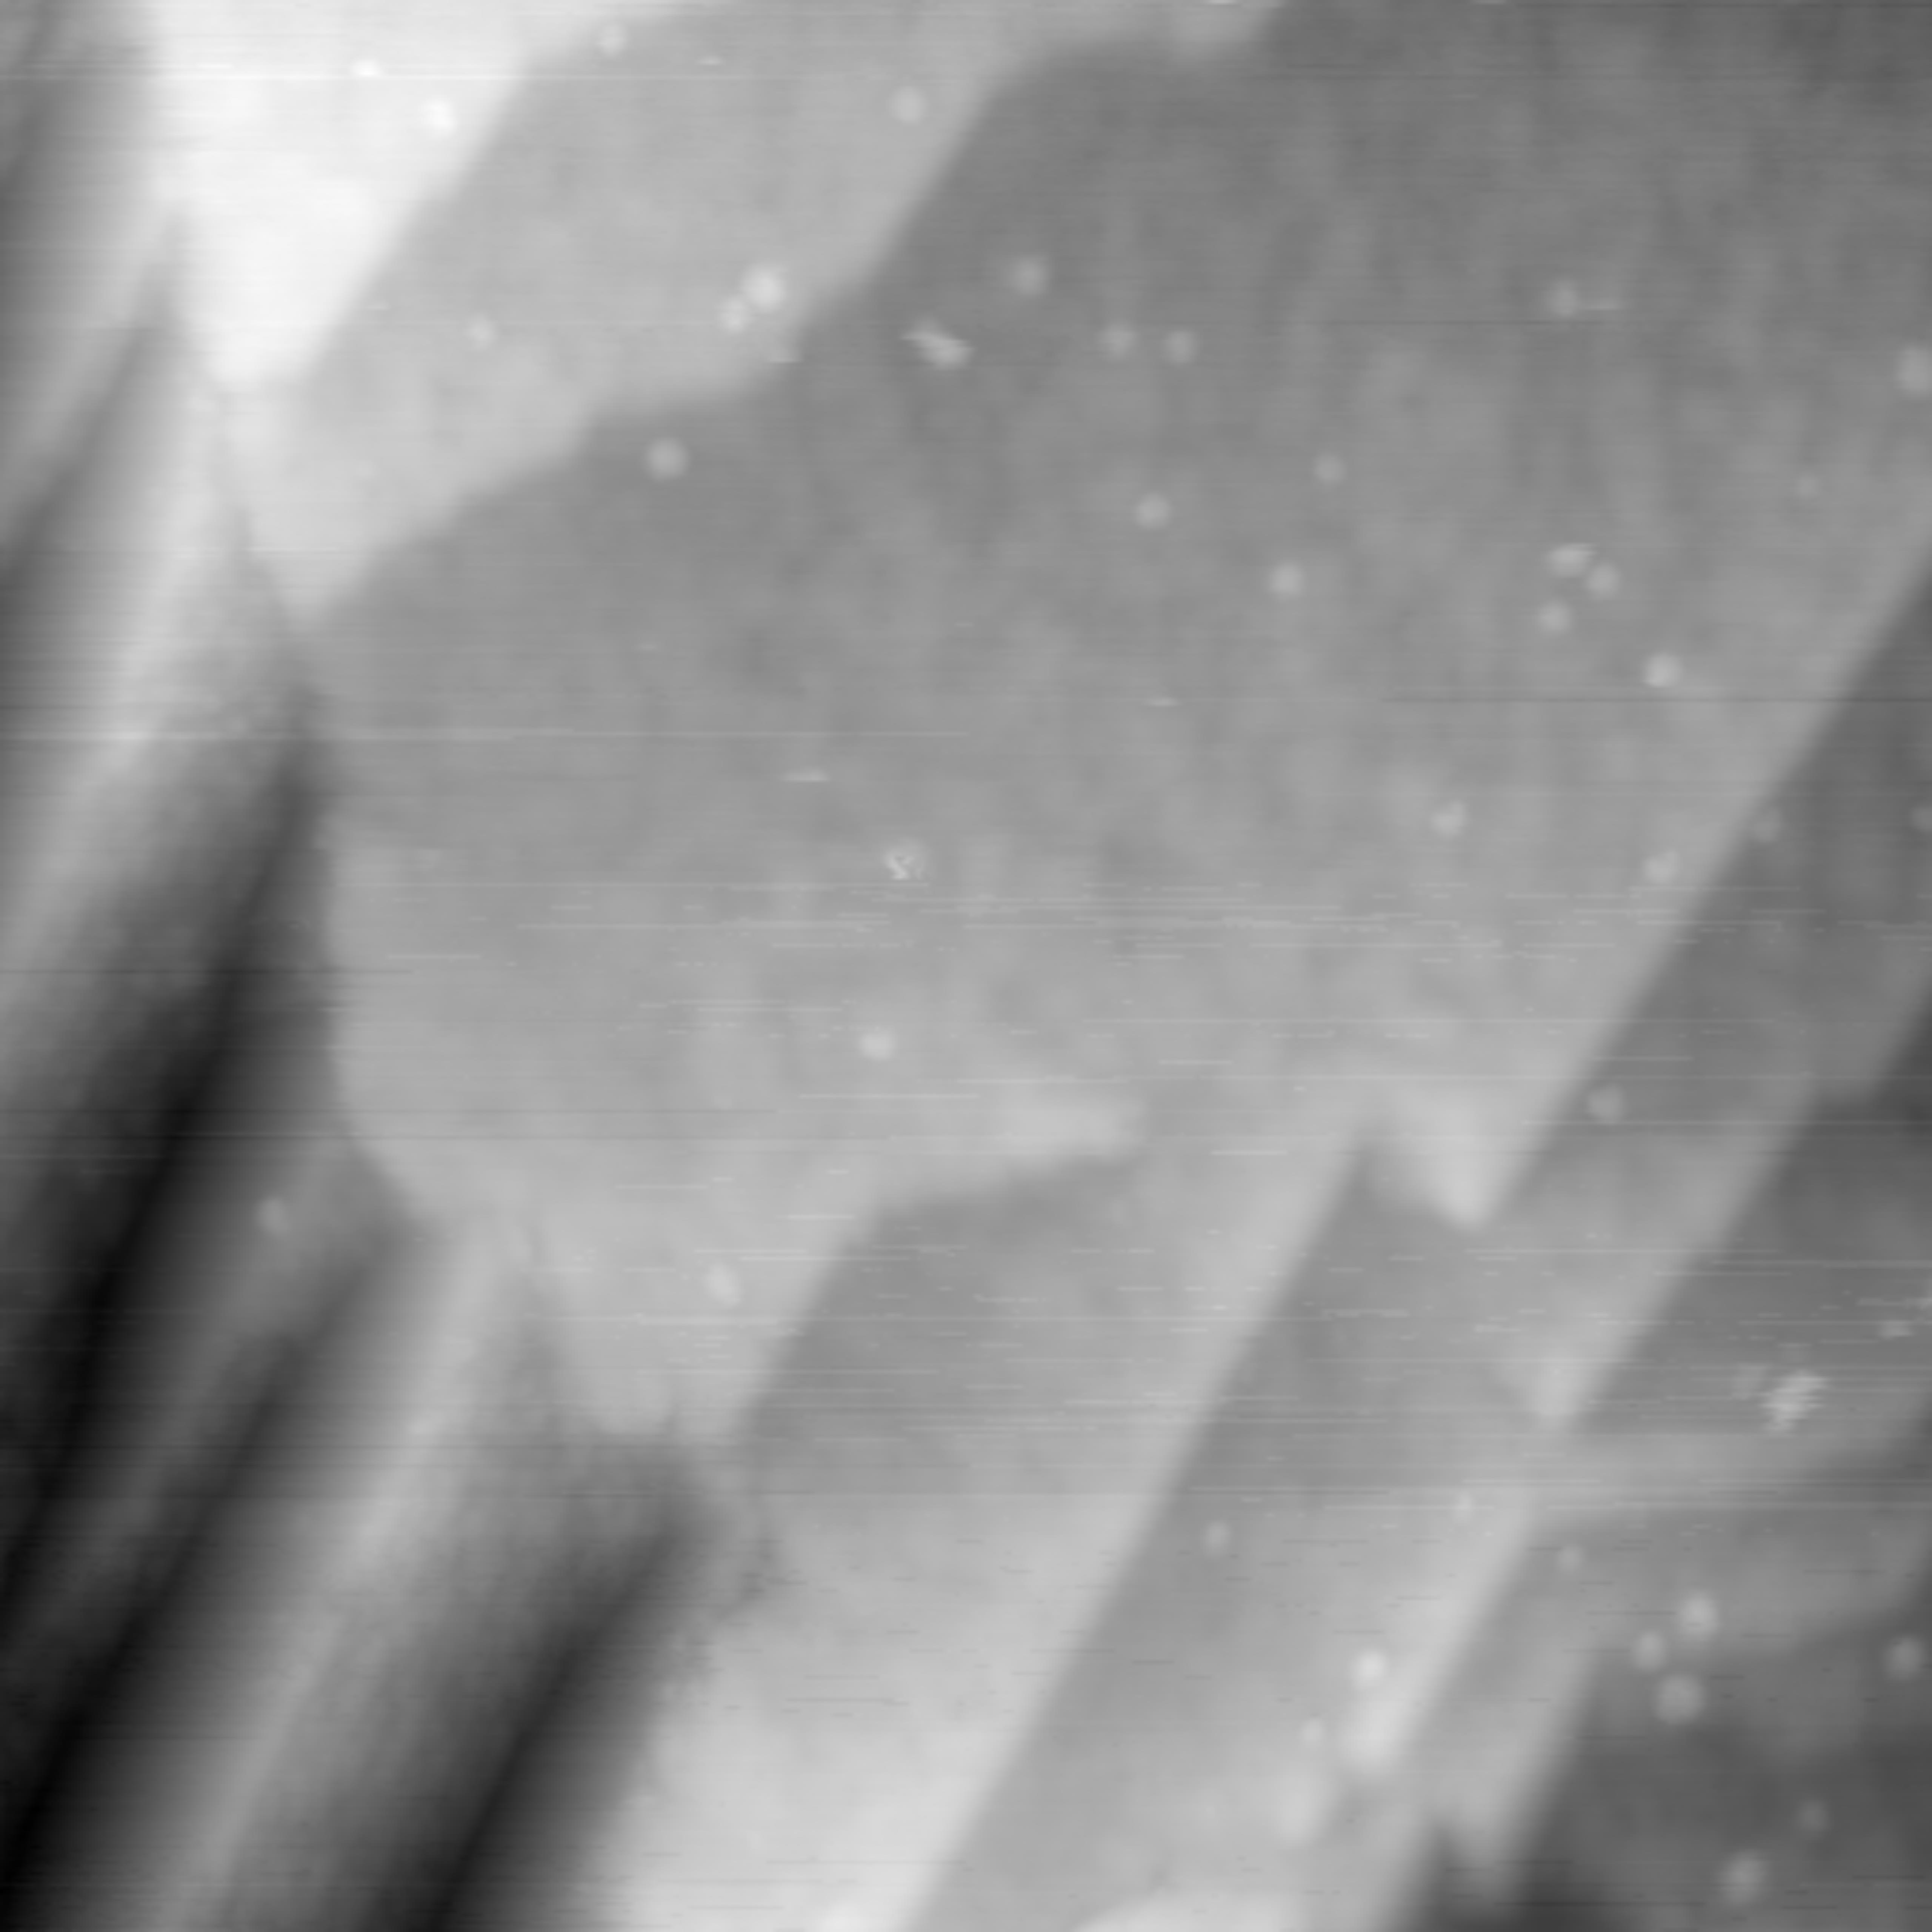
\includegraphics[width=0.45\textwidth]{./images/F150423-114214.jpg} 
% 	\label{fig:h-bn-overgrown-cu-2}
%}%
%\caption{STM topographies of \textit{h}-BN islands that overgrow Cu-foil facets. Imaging parameters: 		
% 	\subref{fig:h-bn-overgrown-cu-1} 
% 		\SI{1}{\volt}, \SI{0.37}{\nano\ampere}, 
% 		color scale \SIrange{0}{1.5}{\nano \meter}, 
% 		Image width: \SI{18}{\nano \meter}, 
% 	\subref{fig:h-bn-overgrown-cu-2} 
% 		\SI{3.5}{\volt}, \SI{0.5}{\nano\ampere}, 
% 		color scale \SIrange{0}{4}{\nano \meter}, 
% 		Image width: \SI{73,8}{\nano \meter}. 
%}%
%\label{fig:h-bn-overgrown-cu}
%\end{figure}

\begin{itemize}
	\item The sample was sputtered and annealed several times to temperatures of \SI{800}{\celsius}. Before the dosage it was held 5 minutes at \SI{750}{\celsius}. Borazine was dosed with the same pressure as before (\SI{1e-7}{\milli \bar}) but for 1min and at a lower temperature of \SI{750}{\celsius}. After the preparation the sample was kept at \SI{750}{\celsius} for another 1 minute. It was cooled down slowly (shown in \autoref{fig:F150416-192611} and \autoref{fig:h-bn-overgrown-cu}).
\end{itemize} 
\begin{figure}
	\centering
	\subfigure[]{%
		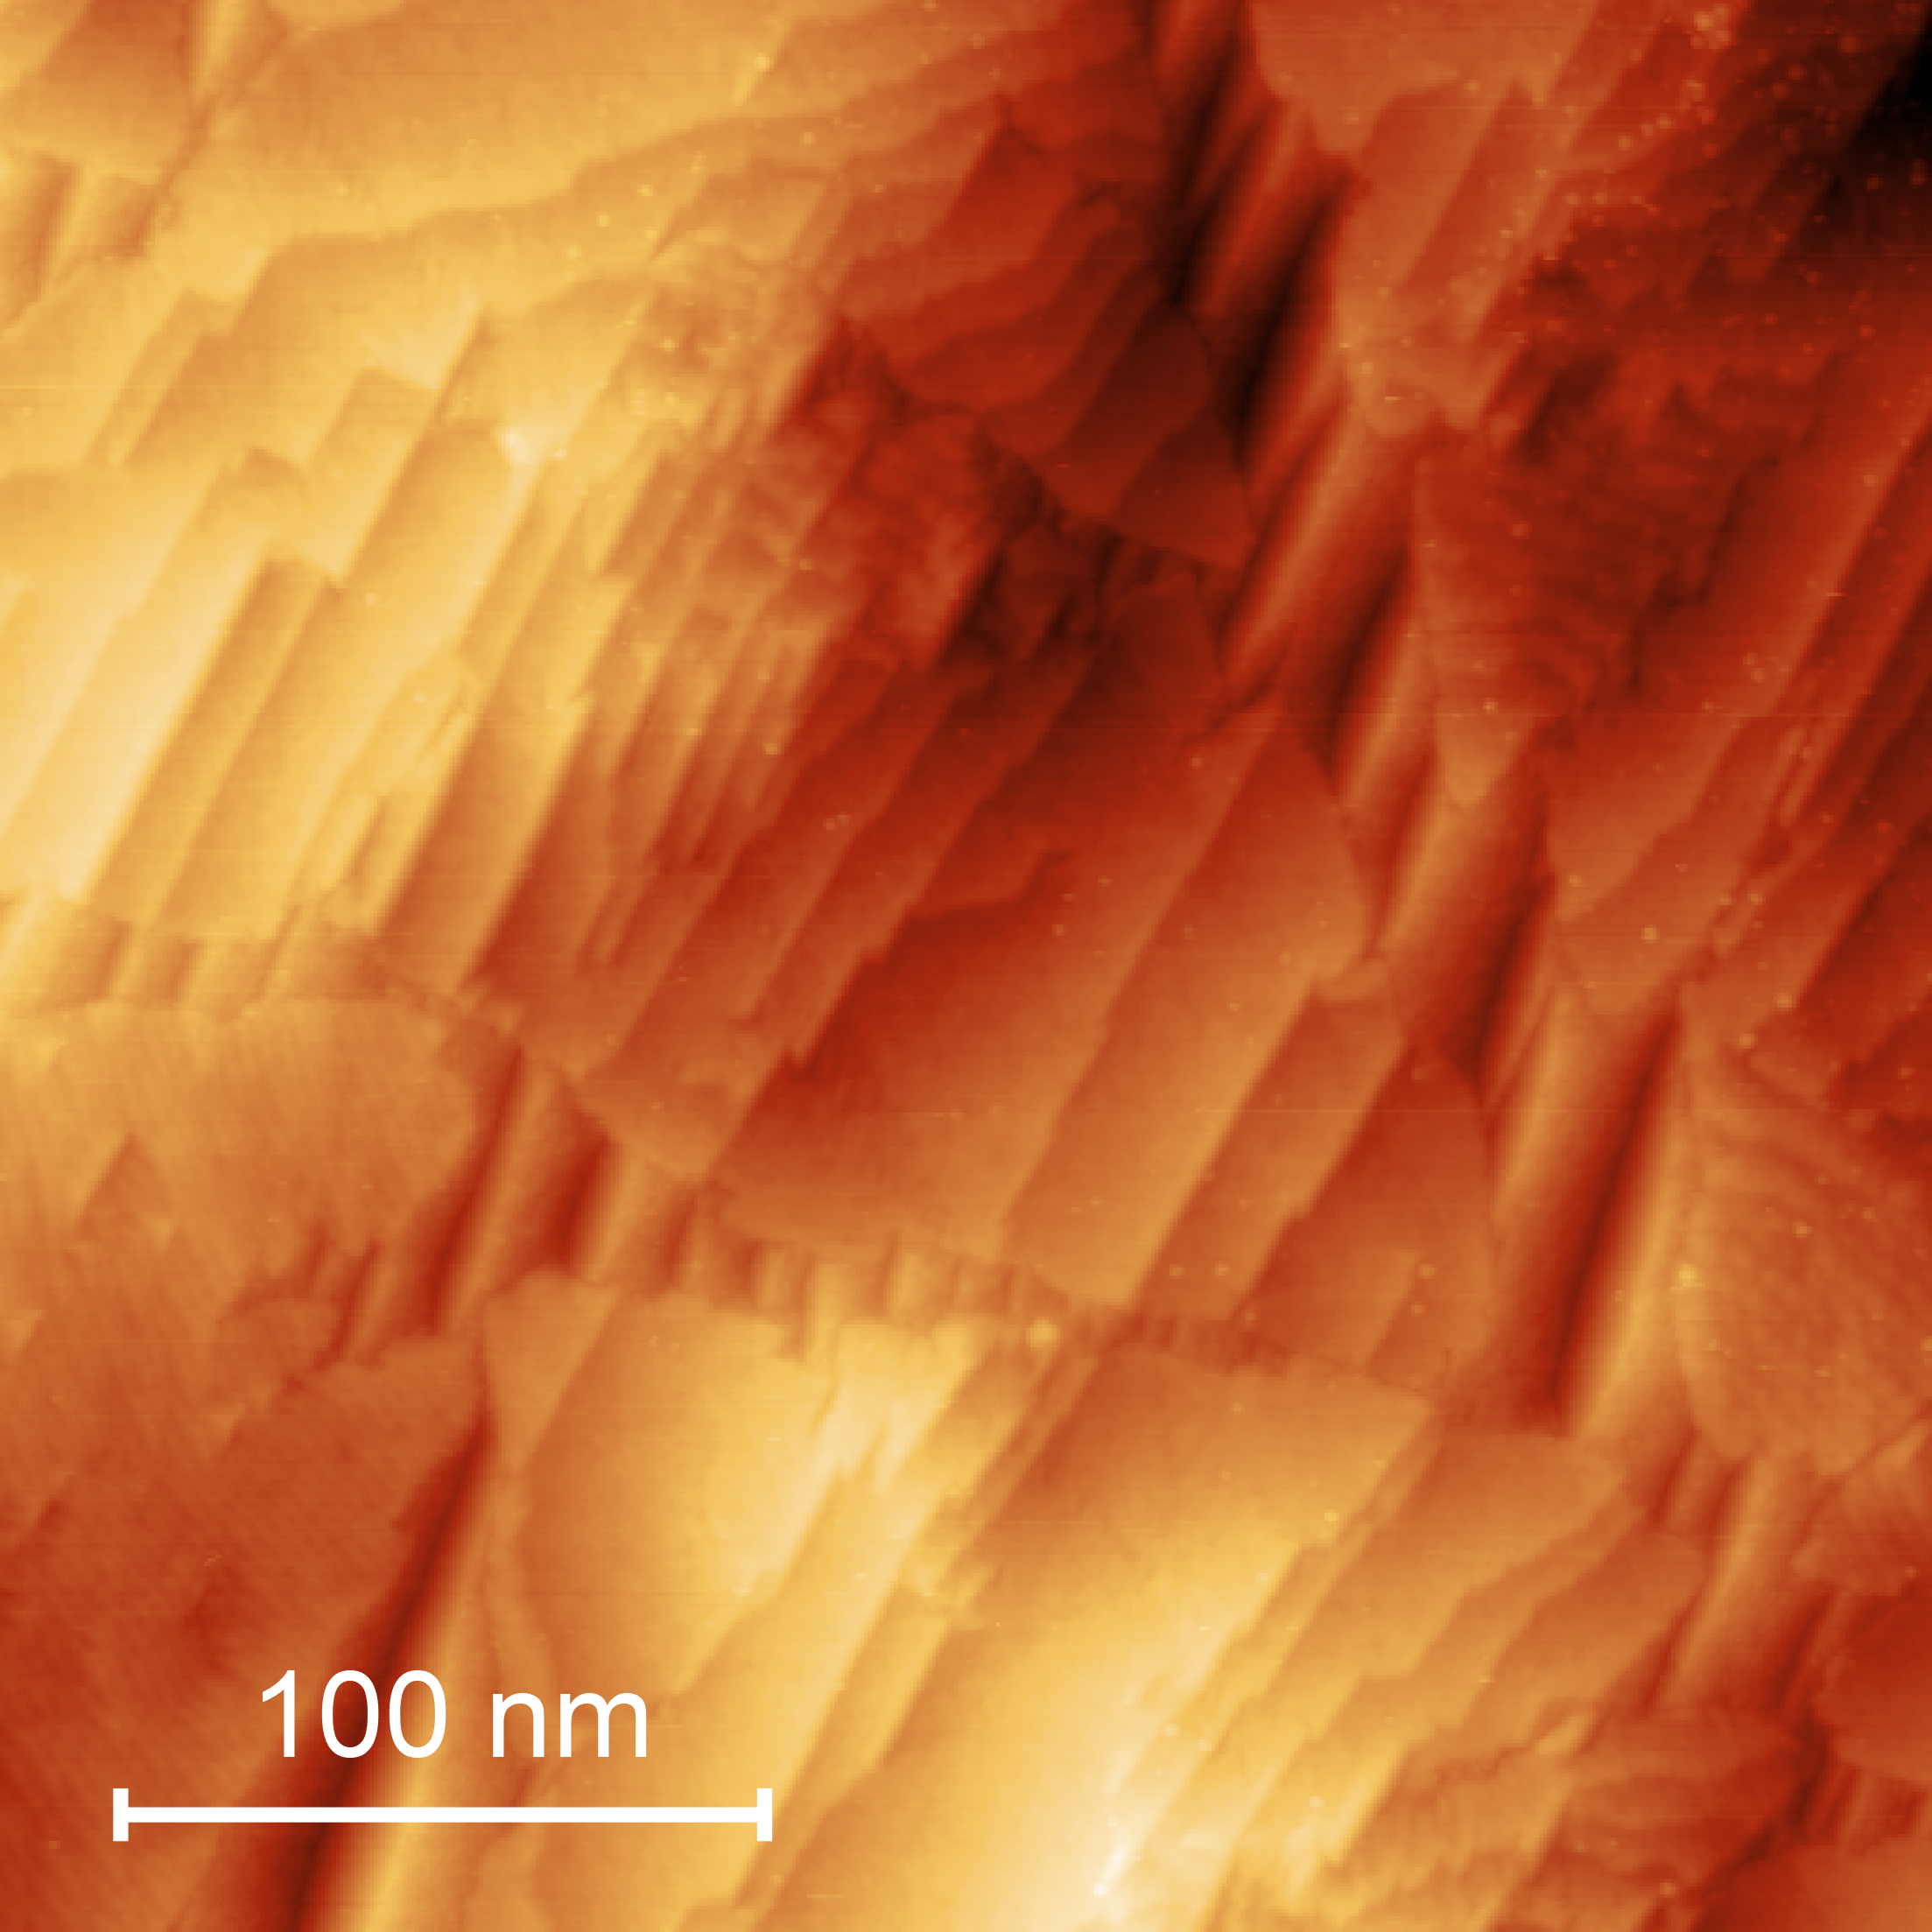
\includegraphics[width=0.45\textwidth]{./images/F150423-102732}
		\label{fig:h-bn-22L}
	} \quad %
	\subfigure[]{%
		\includegraphics[width=0.45\textwidth]{./images/F150423-102732-overlayed.png} 
		\label{fig:h-bn-22L-2}
	}%
	\caption{STM topographies of \textit{h}-BN islands that overgrow Cu-foil facets. Imaging parameters: 		
\SI{4.7}{\volt}, \SI{0.2}{\nano\ampere}, color scale \SIrange{0}{7}{\nano\meter}, Image width: \SI{295}{\nano \meter}
	}%
	\label{fig:h-bn-overgrown-cu}
\end{figure}
%%%%%%%%%%%%%%%%%%%%%%%%%%%%%%%%%%%%%%%%%%%%%%%%%%%%%%%%%%%%%%%%%%%%%%%%%%%%%%%%%%%%%%%%%%
points to point out:
\begin{itemize}
 \item Look at Messzeit-April.ppt power point presentation
 \item Stufenh\"ohe
 \item Beschaffenheit der stufen/facetts $\rightarrow$ material transport mechanism/strength differs under the h-BN compared to the bare cu-foil surface.
 \item Wechselwirkung BN-Wachstum und Facettenbildung
\end{itemize}


\paragraph{surface structure of \textit{h}-BN on Cu-foil}
During experiments some ``new'' structure appeared (compare figure \ref{fig:tpcn-on-cu-foil}).
The apparent height change between the both terraces is \SI{130}{\pico \meter} separated by a slim trench that is slightly lower than the right terrace (\SI{50}{\pico \meter}). The parallel stripes have an apparent corrugation of \SI{25}{\pico \meter} and are separated \SI{70}{\pico \meter} from each other and cover the whole image. 

The adsorbed TPCN molecules show different apparent heights in their molecular center. Some fragmented and heavily deformed molecules are visible.

\begin{figure}
 \centering
 \subfigure[Molecules on copper foil surface - supposed be be covered with \textit{h}-BN, maybe just free (maybe facetted) copper. Stripes not visible on the lower teracce, although present in the same orientation.]{
 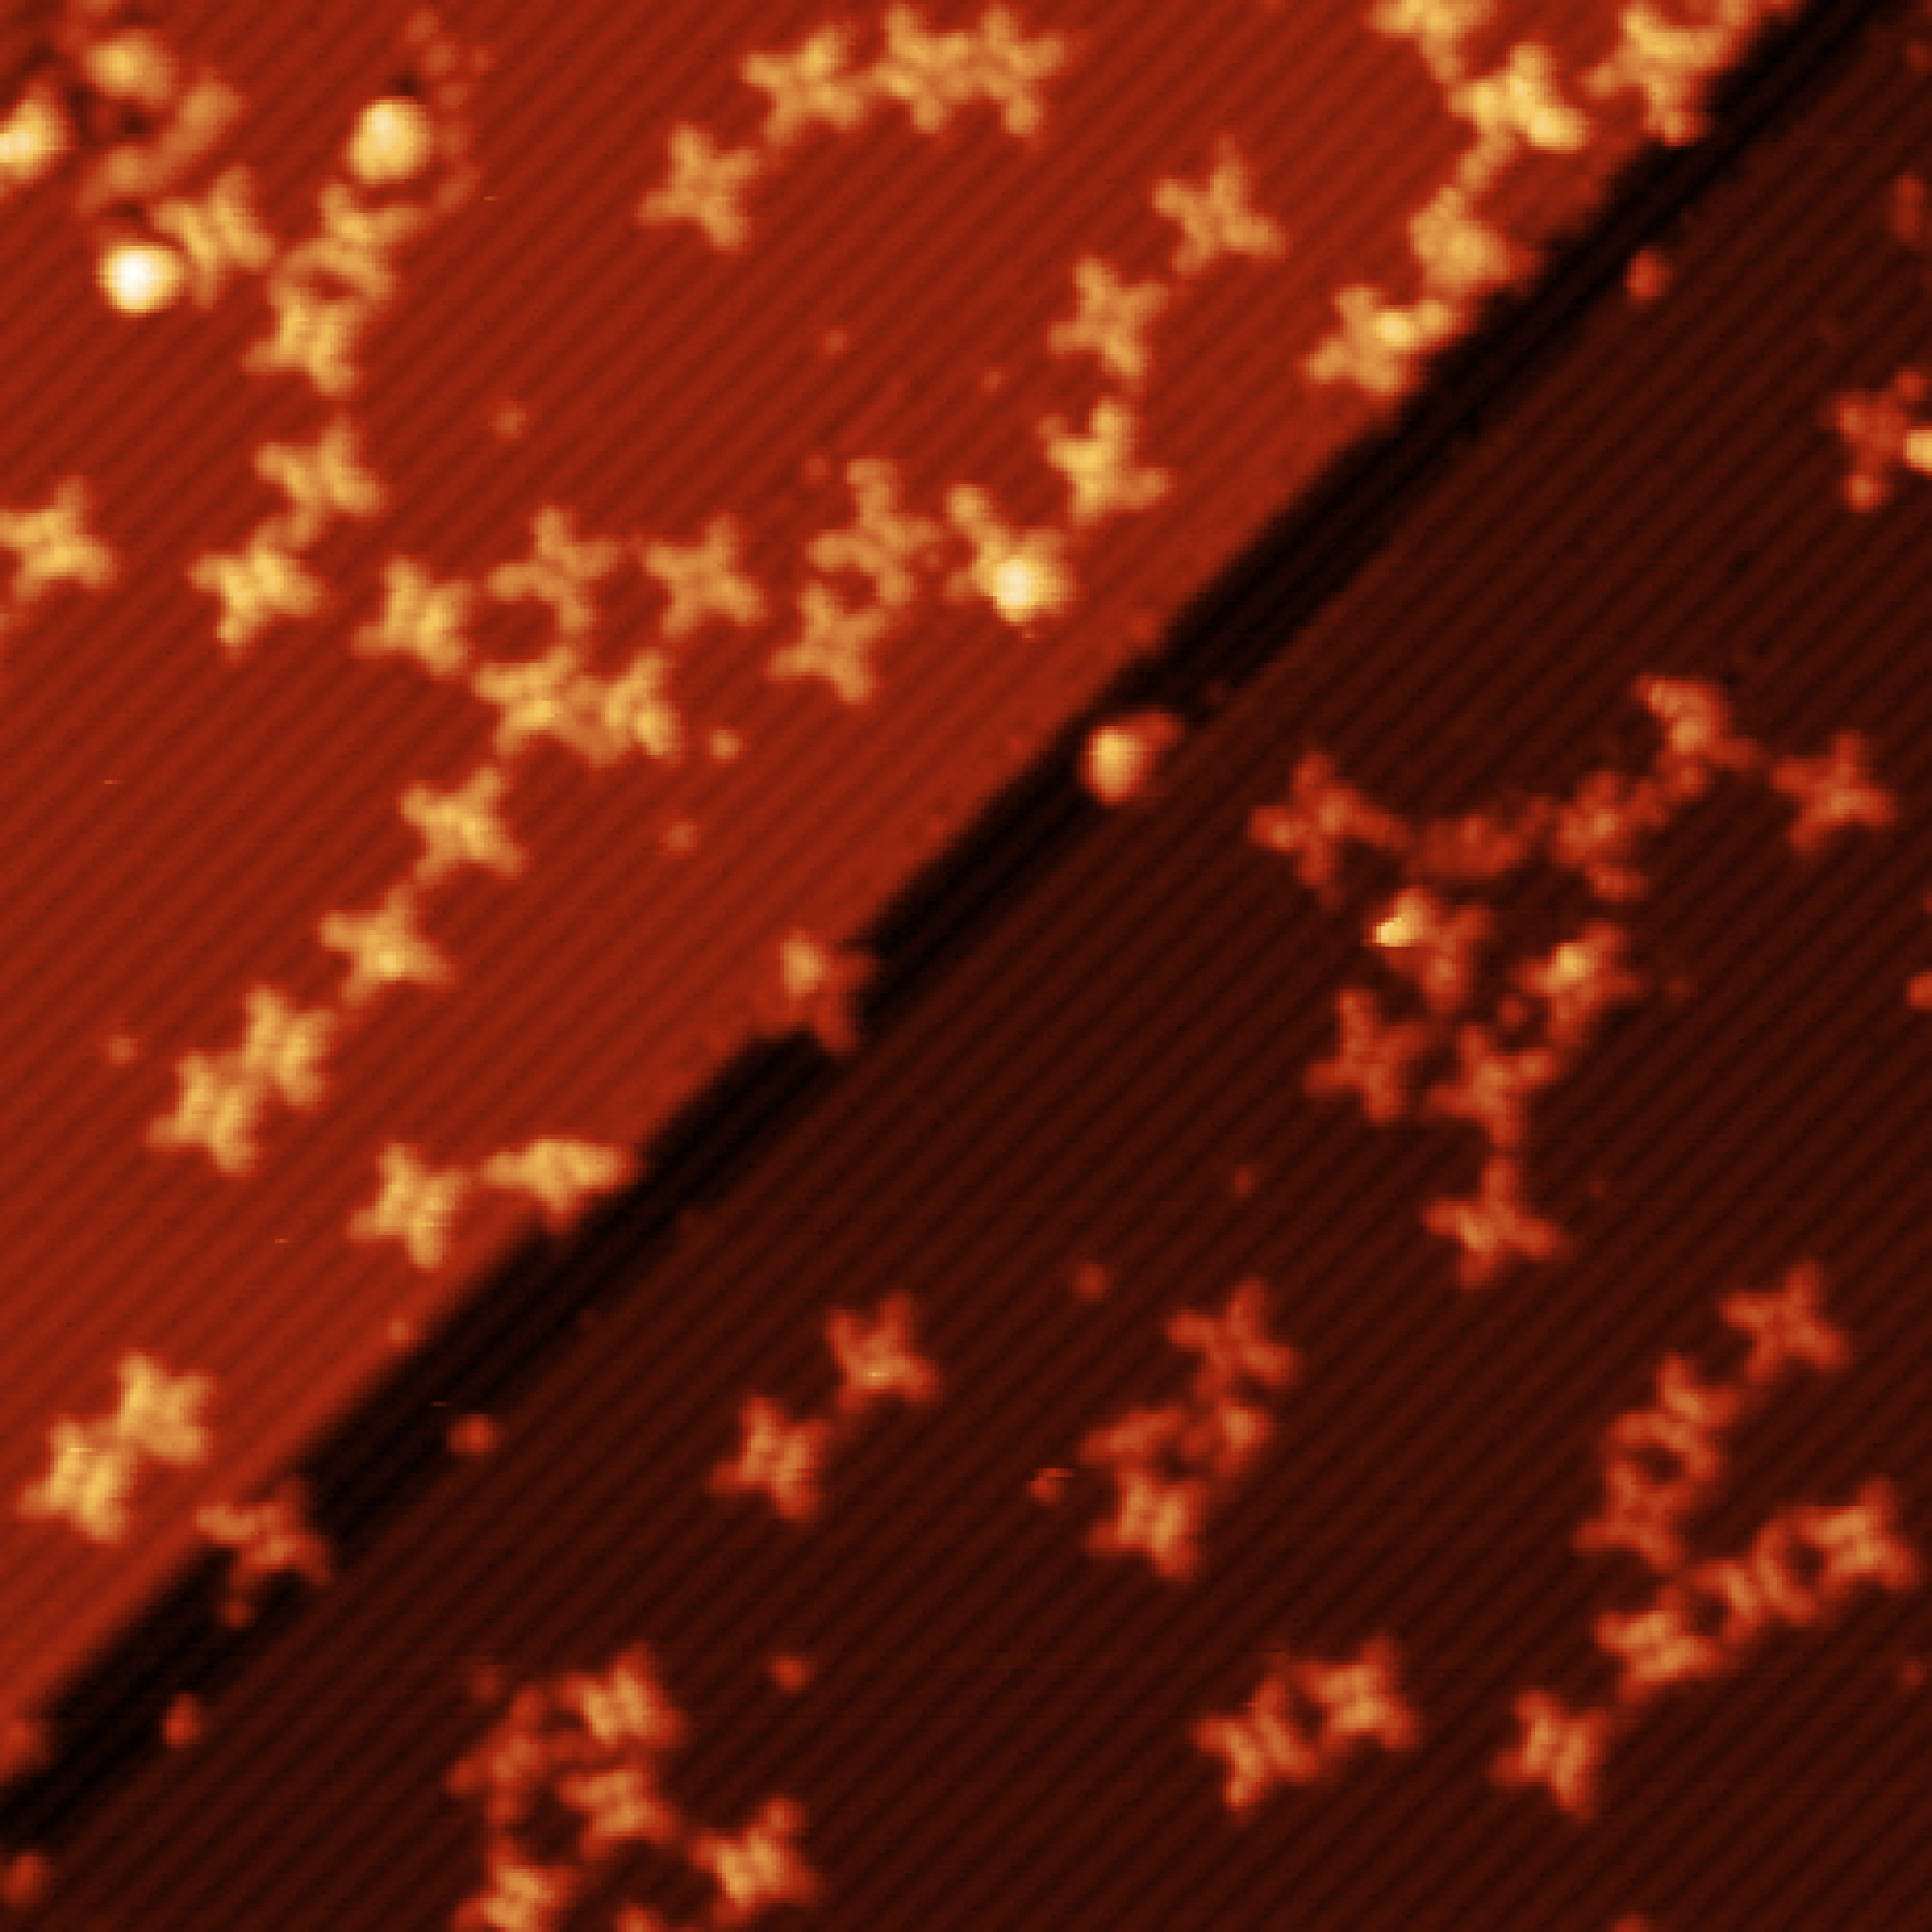
\includegraphics[width=0.45\textwidth]{./images/F150810-113456}
 \label{fig:tpcn-on-cu-foil-stm}
 } \quad
 \subfigure[Line spectrum across the step shown in \subref{fig:tpcn-on-cu-foil-stm} perpendicular to the trench. No molecules were crossed.]{
	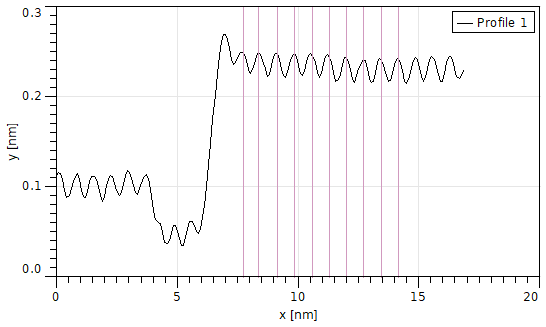
\includegraphics[width=0.45\textwidth]{./images/F150810-113456-line-spectra}
\label{fig:tpcn-on-cu-foil-spectrum}
}
 \caption{Surface structure of copper foil after deposition of TPCN molecules. Two terraces are visible, both covered with linear stripes - oxygen over layer (2x1)?- cu reconstruction? - maybe some very small (\SI{0.75}{\nm}) linear moire on a Cu(100) facet? Noise can be excluded due to the fact that the stripes do not occur on the molecules, but only on the substrate. Adsorbed TPCN molecules appear as cross shaped protrusions. Many deformed molecular cores visible throughout the image $\rightarrow$ strong substrate interaction $\rightarrow$ no \textit{h}-BN! Line spectrum shown in \subref{fig:tpcn-on-cu-foil-spectrum} indicating a period of \SI{70}{\pico \meter}. Imaging parameters: 		
 	\subref{fig:tpcn-on-cu-foil-stm} 
 	\SI{1.26}{\volt}, \SI{0.04}{\nano\ampere}, 
 	color scale \SIrange{0}{0.8}{\nano \meter}, 
 	Image width: \SI{40}{\nano \meter} }
\label{fig:tpcn-on-cu-foil}
\end{figure}
